\documentclass[12pt, a4paper, oneside]{ctexart}
\usepackage{amsmath, amsthm, amssymb, bm, color, graphicx, geometry, hyperref, mathrsfs,extarrows, braket}

\linespread{1.5}
\geometry{left=2.54cm,right=2.54cm,top=3.18cm,bottom=3.18cm}
\newenvironment{problem}{\par\noindent\textbf{题目. }}{\bigskip\par}
\newenvironment{solution}{\par\noindent\textbf{解答. }}{\bigskip\par}
\newenvironment{note}{\par\noindent\textbf{注记. }}{\bigskip\par}

% 基本信息
\newcommand{\dt}{\today}
\newcommand{\sj}{离散数学}
\newcommand{\vt}{吴天阳 2204210460}

\begin{document}

\pagestyle{empty}
\vspace*{-20ex}
\centerline{\begin{tabular}{*3{c}}
    \parbox[t]{0.3\linewidth}{\begin{center}\textbf{日期}\\ \large \textcolor{blue}{\dt}\end{center}} 
    & \parbox[t]{0.3\linewidth}{\begin{center}\textbf{科目}\\ \large \textcolor{blue}{\sj}\end{center}}
    & \parbox[t]{0.3\linewidth}{\begin{center}\textbf{姓名,学号}\\ \large \textcolor{blue}{\vt}\end{center}} \\ \hline
\end{tabular}}
\vspace*{4ex}
\paragraph{习题八}
\paragraph{32.}\begin{proof}
    设图$G$为小于$30$条边的平面简单图,含有$n$个结点$m$条边$r$个区域,由于$G$为简单图,所以没有自环与重边。
    
    反设$G$中结点的度数均大于等于$5$,由于一条边含有两个端点,则
    \begin{equation}
        m\geqslant \frac{5}{2}n
    \end{equation}
    由于$G$为平面图,由$\text{Euler}$公式,知
    \begin{equation*}
        n-m+r=2
    \end{equation*}
    又由于$G$不含重边与自环,所以每个区域至少由三条边围成,且每一条边至多为两个区域的公共边,则
    \begin{equation*}
        \begin{aligned}
        &\ r\leqslant \frac{2}{3}m\\
        \Rightarrow&\ m-n+2\leqslant\frac{2}{3}m\\
        \Rightarrow&\begin{cases}
            m\leqslant 3n-6\\
            m\geqslant\dfrac{5}{2}n&\text{条件}(1)
        \end{cases}\\
        \Rightarrow&\ 
            m\geqslant 30
        \end{aligned}
    \end{equation*}
    与$m < 30$矛盾,综上,一定存在至少一个结点的度数小于等于$4$。
\end{proof}
\newpage
\paragraph{34.}\begin{solution} 如图所示:

    \centerline{
        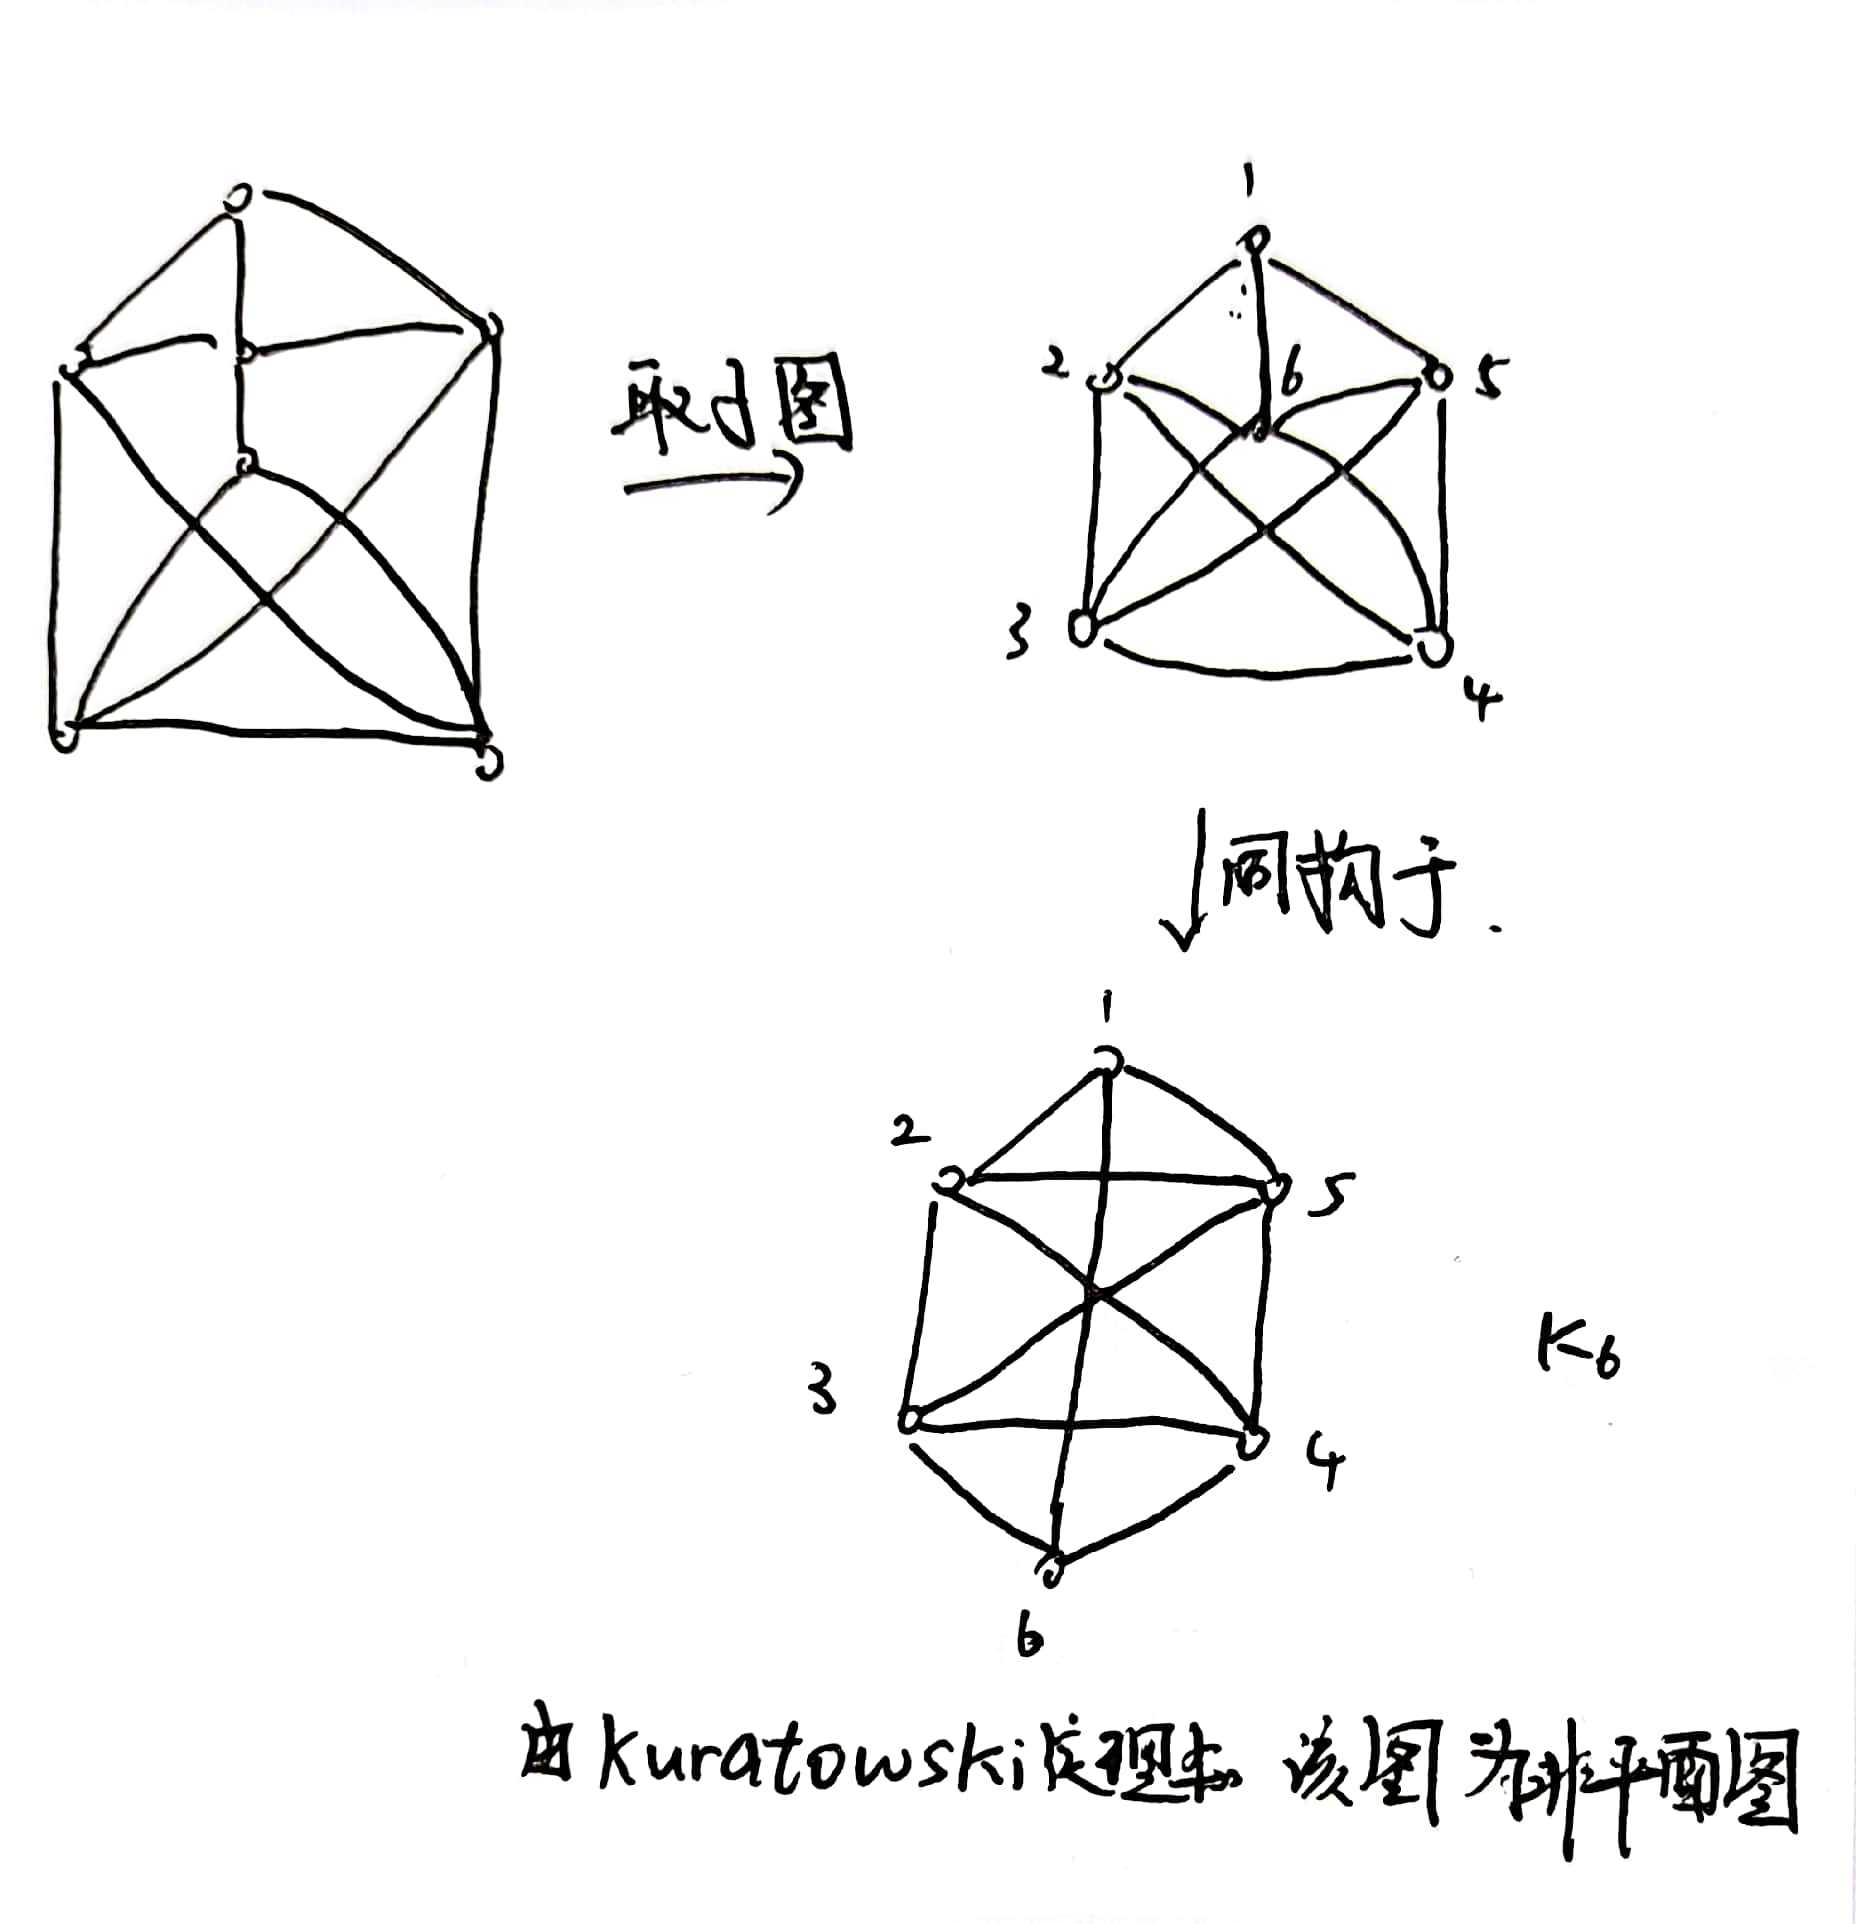
\includegraphics[width=0.6\textwidth]{graph1.jpg}
    }
\end{solution}
\end{document}
